\documentclass{article}
\usepackage[utf8]{inputenc}
\usepackage{graphicx}
\usepackage{amsmath}
\usepackage{caption}
\usepackage{neuralnetwork}
\usepackage{float} 
\usepackage{lipsum}  % For dummy text
\usepackage{listings}
\usepackage{xcolor}
\usepackage{tocloft}
\usepackage{hyperref}
\usepackage{tikz}
\usetikzlibrary{positioning,shapes}

\usetikzlibrary{positioning, arrows.meta, shapes.geometric}

\definecolor{codegreen}{rgb}{0,0.6,0}
\definecolor{codegray}{rgb}{0.5,0.5,0.5}
\definecolor{codepurple}{rgb}{0.58,0,0.82}
\definecolor{backcolour}{rgb}{0.95,0.95,0.92}


\lstdefinestyle{mystyle}{
    backgroundcolor=\color{backcolour},
    commentstyle=\color{codegreen},
    keywordstyle=\color{magenta},
    numberstyle=\tiny\color{codegray},
    stringstyle=\color{codepurple},
    basicstyle=\ttfamily,
    breakatwhitespace=false,
    breaklines=true,
    captionpos=b,
    keepspaces=true,
    showspaces=false,
    showstringspaces=false,
    showtabs=false,
    tabsize=2
}



% Redefine the abstract environment
\renewenvironment{abstract}
 {\small\quotation\noindent\ignorespaces}
 {\endquotation}

\begin{document}

\begin{titlepage}
  \centering
 \vspace*{\fill}
  \includegraphics[width=\textwidth]{university_logo.png}  
 \vspace*{\fill}
  \title{Demystifying Shape Recognition with Simplified Neural Networks: A Deep Dive into Code and Concepts}
  \author{Ankit Ankit s0580270}
  \date{\ February 10, 2024 }
  \maketitle

\begin{abstract}
This paper dissects the intricacies of a simplified neural network designed for basic shape recognition. Through meticulous code analysis, the paper unveils the network's core functionalities, training mechanisms, and learning capabilities. By exploring the model's strengths and limitations, the paper illuminates its potential as a stepping stone towards comprehending more intricate neural networks and their applications in visual recognition.
\end{abstract}
\end{titlepage}
\clearpage

\tableofcontents

\clearpage
\section{Introduction}
Have you ever wondered how machines learn to recognize shapes or patterns? Neural networks, inspired by the human brain's ability to recognize patterns, have revolutionized various fields. However, their complex architectures can pose a significant barrier to understanding their inner workings, especially for beginners. This paper delves into the inner workings of a simplified neural network designed for a specific task: recognizing basic shapes like squares and circles.

\section*{By meticulously dissecting the code, the paper aims to:}
\begin{itemize}
    \item Unveil the network's core functionalities: Explain how the network represents layers and weights, how information flows through the network, and how it uses this information to make predictions.
    \item Demystify the training mechanisms: Explore how the network learns by adjusting its weights based on feedback from its environment.
    \item Evaluate the learning capabilities: Analyze the network's performance in recognizing shapes and discuss its limitations compared to more complex models.
    \item Position the model as a learning tool: Highlight the value of this simplified model as an educational tool for understanding the fundamental principles of neural networks before venturing into more intricate architectures.
\end{itemize}
Through this exploration, the paper aims to demystify the underlying concepts of neural networks and showcase their potential in visual recognition tasks. This understanding serves as a stepping stone for further exploration of more complex models and their diverse applications.

\begin{figure}[H]  
  \centering
  \includegraphics[width=0.406\textwidth]{ifs-40-ifs189212-g003}  
  \caption{Basic Neural Network}  
\end{figure}

\section{Code Analysis and Functionality}

\subsection{Data Structures}
The code represents layers and weights using two-dimensional arrays of floating-point numbers. This choice aligns with the matrix-based operations often employed in neural networks. The `typedef` declaration creates a convenient alias, `Layer`, for these arrays, enhancing code readability.

\lstset{language=C, breaklines=true, basicstyle=\ttfamily}
\begin{lstlisting}
typedef float Layer[HEIGHT][WIDTH];

// function to access weight at specific row and column
float get\_weight(Layer weights, int y, int x) {
  return weights[y][x];
}
\end{lstlisting}

\section*{Key observations:}
\begin{itemize}
  

    \item Floating-point precision: The use of `float` data type offers a balance between precision and memory efficiency. It's often sufficient for representing weights in neural networks without excessive memory consumption
    \item Array-based structure: Arrays provide efficient access to elements, crucial for matrix multiplications and other vectorized operations common in neural network computations.
    \item Direct weight access: The `get\_weight` function demonstrates how individual weights can be retrieved using their row and column indices. This enables fine-grained manipulation of weights during training and inference.
    \end{itemize}

\section*{Considerations:}
\begin{itemize}
    \item  Memory requirements: While arrays offer efficient access, they can become memory-intensive for large networks. Careful memory management might be necessary to accommodate large models.
    \item  Alternative data structures: In specific scenarios, other data structures like sparse matrices or tensors might offer advantages in terms of memory usage or computational efficiency, depending on the network's architecture and operations.
\end{itemize}
\clearpage
\section{Functions}

\subsection*{\texttt{clampi}}

\textbf{Description:} This function clamps an integer value within a specified range.

\textbf{Parameters:}
\begin{itemize}
    \item \texttt{x} (int): Value to be clamped.
    \item \texttt{low} (int): Lower bound of the range.
    \item \texttt{high} (int): Upper bound of the range.
\end{itemize}

\subsection*{\texttt{layer\_save\_as\_csv}}

\textbf{Description:} Saves the weights of a layer to a CSV file.

\textbf{Parameters:}
\begin{itemize}
    \item \texttt{layer} (Layer): The 2D array representing the layer.
    \item \texttt{file\_path} (const char*): The path to the CSV file.
\end{itemize}

\subsection*{\texttt{layer\_load\_from\_csv}}

\textbf{Description:} Loads weights from a CSV file into a layer.

\textbf{Parameters:}
\begin{itemize}
    \item \texttt{weights} (Layer): The 2D array to store the loaded weights.
    \item \texttt{file\_path} (const char*): The path to the CSV file.
\end{itemize}

\subsection*{\texttt{layer\_fill\_rect}}

\textbf{Description:} Fills a rectangular region in a layer with a specified value.

\textbf{Parameters:}
\begin{itemize}
    \item \texttt{layer} (Layer): The 2D array representing the layer.
    \item \texttt{x}, \texttt{y} (int): Coordinates of the top-left corner of the rectangle.
    \item \texttt{w}, \texttt{h} (int): Width and height of the rectangle.
    \item \texttt{value} (float): The value to fill the rectangle with.
\end{itemize}

\subsection*{\texttt{layer\_fill\_circle}}

\textbf{Description:} Fills a circular region in a layer with a specified value.

\textbf{Parameters:}
\begin{itemize}
    \item \texttt{layer} (Layer): The 2D array representing the layer.
    \item \texttt{cx}, \texttt{cy} (int): Coordinates of the circle's center.
    \item \texttt{r} (int): Radius of the circle.
    \item \texttt{value} (float): The value to fill the circle with.
\end{itemize}

\subsection*{\texttt{layer\_save\_as\_ppm}}

\textbf{Description:} Saves a layer as a PPM (Portable Pixmap) image file.

\textbf{Parameters:}
\begin{itemize}
    \item \texttt{layer} (Layer): The 2D array representing the layer.
    \item \texttt{file\_path} (const char*): The path to the PPM file.
\end{itemize}

\subsection*{\texttt{layer\_save\_as\_bin}}

\textbf{Description:} Saves a layer to a binary file.

\textbf{Parameters:}
\begin{itemize}
    \item \texttt{layer} (Layer): The 2D array representing the layer.
    \item \texttt{file\_path} (const char*): The path to the binary file.
\end{itemize}

\subsection*{\texttt{layer\_load\_from\_bin}}

\textbf{Description:} Loads a layer from a binary file.

\textbf{Parameters:}
\begin{itemize}
    \item \texttt{layer} (Layer): The 2D array to store the loaded layer.
    \item \texttt{file\_path} (const char*): The path to the binary file.
\end{itemize}

\subsection*{\texttt{add\_inputs\_from\_weights}}

\textbf{Description:} Adds the values of one layer to another.

\textbf{Parameters:}
\begin{itemize}
    \item \texttt{inputs}, \texttt{weights} (Layer): The 2D arrays representing layers.
\end{itemize}

\subsection*{\texttt{sub\_inputs\_from\_weights}}

\textbf{Description:} Subtracts the values of one layer from another.

\textbf{Parameters:}
\begin{itemize}
    \item \texttt{inputs}, \texttt{weights} (Layer): The 2D arrays representing layers.
\end{itemize}

\subsection*{\texttt{rand\_range}}

\textbf{Description:} Generates a random integer within a specified range.

\textbf{Parameters:}
\begin{itemize}
    \item \texttt{low}, \texttt{high} (int): The range within which the random integer is generated.
\end{itemize}

\subsection*{\texttt{layer\_random\_rect}}

\textbf{Description:} Fills a layer with a random rectangular pattern.

\textbf{Parameters:}
\begin{itemize}
    \item \texttt{layer} (Layer): The 2D array representing the layer.
\end{itemize}

\subsection*{\texttt{layer\_random\_circle}}

\textbf{Description:} Fills a layer with a random circular pattern.

\textbf{Parameters:}
\begin{itemize}
    \item \texttt{layer} (Layer): The 2D array representing the layer.
\end{itemize}

\subsection*{\texttt{feed\_forward}}

\textbf{Description:} Performs the feedforward step of the neural network.

\textbf{Parameters:}
\begin{itemize}
    \item \texttt{inputs}, \texttt{hidden\_weights}, \texttt{output\_weights} (Layer): The 2D arrays representing layers.
\end{itemize}

\subsection*{\texttt{train\_pass}}

\textbf{Description:} Conducts a training pass on the neural network.

\textbf{Parameters:}
\begin{itemize}
    \item \texttt{inputs}, \texttt{hidden\_weights}, \texttt{output\_weights} (Layer): The 2D arrays representing layers.
\end{itemize}

\subsection*{\texttt{check\_pass}}

\textbf{Description:} Checks the performance of the neural network on a set of random patterns.

\textbf{Parameters:}
\begin{itemize}
    \item \texttt{inputs}, \texttt{hidden\_weights}, \texttt{output\_weights} (Layer): The 2D arrays representing layers.
\end{itemize}

\subsection*{\texttt{main}}

\textbf{Description:} The main function orchestrating the execution of the entire program.

\textbf{No Parameters.}


\section{Feedforward Mechanism}

This section provides a detailed overview of how input data moves through the neural network, interacts with weights, and ultimately produces an output:



\begin{enumerate}
    \item \textbf{Inputs Propagation:} Input values traverse the neural network by interacting with hidden layer weights, where each input is multiplied by its corresponding weight, and the results contribute to the hidden layer's output.

    \item \textbf{Activation and Output:} The hidden layer's output undergoes activation using a step function, determining if it surpasses a predefined bias. The activated output is then combined with output layer weights, producing the final output of the neural network for shape recognition.
\end{enumerate}



\lstset{language=C, breaklines=true, basicstyle=\ttfamily}
\begin{lstlisting}
float feed_forward(Layer inputs, Layer hidden_weights, Layer output_weights) {
    float hidden_output = 0.0f;
    #pragma omp parallel for reduction(+:hidden_output)
    for (int y = 0; y < HEIGHT; ++y) {
        #pragma omp simd for (int x = 0; x < WIDTH; ++x) {
            hidden_output += inputs[y][x] * hidden_weights[y][x];
        }
    }
    // a step function as the activation function for simplicity
    float hidden_activation = (hidden_output > BIAS) ? 1.0f : 0.0f;
    float final_output = 0.0f;
    #pragma omp parallel for reduction(+:final_output)
    for (int y = 0; y < HEIGHT; ++y) {
        #pragma omp simd for (int x = 0; x < WIDTH; ++x) {
            final_output += hidden_activation * output_weights[y][x];
        }
    }
    return final_output;
}
\end{lstlisting}


\clearpage
\subsection{Layer Management}
There are three layers in this neural network architecture:
\subsubsection{Input Layer}
\begin{itemize}
    \item The network receives an input layer inputs representing the image data (e.g., pixel values).
    \item Each element in inputs corresponds to a pixel in the image.
\end{itemize}
\subsubsection{Hidden Layer}
\begin{itemize}
    \item Each neuron in the hidden layer calculates a weighted sum of its inputs from the input layer.
    \item A non-linear activation function, like a step function in this case, is applied to the weighted sum to introduce non-linearity. This helps the network learn complex relationships between inputs and outputs.  
\end{itemize}

   
 \subsubsection{Output Layer}
    \begin{itemize}
        \item The output neuron calculates a weighted sum of its inputs from the hidden layer.
\item The activation function is again applied to this weighted sum to produce the final output of the network.
          \end{itemize}

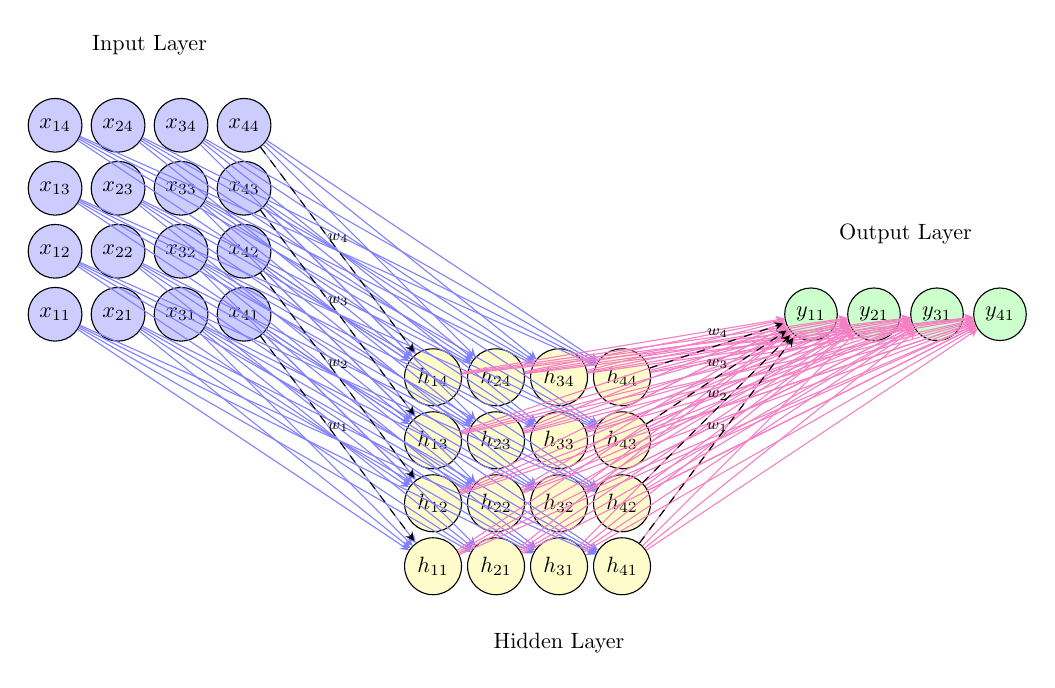
\begin{tikzpicture}[>=stealth, scale=0.8, transform shape]

% Input layer
\foreach \y in {1,...,4}
    \foreach \x in {1,...,4}
        \node[draw,circle,minimum size=0.6cm, fill=blue!20] (I-\x-\y) at (\x, \y+4) {$x_{\x\y}$};

% Hidden layer
\foreach \y in {1,...,4}
    \foreach \x in {1,...,4}
        \node[draw,circle,minimum size=0.6cm, fill=yellow!20] (H-\x-\y) at (\x+6, \y) {$h_{\x\y}$};

% Output layer
\foreach \y in {1,...,1}
    \foreach \x in {1,...,4}
        \node[draw,circle,minimum size=0.6cm, fill=green!20] (O-\x-\y) at (\x+12, \y+4) {$y_{\x\y}$};


% Connections
\foreach \x in {1,...,4}
    \foreach \y in {1,...,4}
        \foreach \z in {1,...,4}
            \draw[->, blue!50] (I-\x-\y) -- (H-\z-\y);

\foreach \x in {1,...,4}
    \foreach \y in {1,...,4}
        \foreach \z in {1,...,4}
            \draw[->, magenta!50] (H-\x-\y) -- (O-\z-1);

% Labels
\node[align=center, above] at (2.5, 9) {Input Layer};
\node[align=center, above] at (9, -0.5) {Hidden Layer};
\node[align=center, above] at (14.5, 6) {Output Layer};

% Connections labels
\foreach \y in {1,...,4}
    \draw[->, dashed, shorten >=1pt] (I-4-\y) -- (H-1-\y) node[midway, above, font=\scriptsize] {$w_{\y}$};

\foreach \y in {1,...,4}
    \draw[->, dashed, shorten >=1pt] (H-4-\y) -- (O-1-1) node[midway, above, font=\scriptsize] {$w_{\y}$};

\end{tikzpicture}
\subsubsection{Calculation of Neurons }
The total number of neurons in the neural network can be calculated as follows:

\begin{itemize}
    \item Input layer: $WIDTH \times HEIGHT = 20 \times 20 = 400$ neurons
    \item Hidden layer: $HIDDEN\_SIZE = 64$ neurons
    \item Output layer: $OUTPUT\_SIZE = 1$ neuron
\end{itemize}

Therefore, the total number of neurons is given by:
\[
\text{Total neurons} = 400 + 64 + 1 = 465
\]
\subsection{Feedforward Journey}
\subsubsection*{Hidden Layer Weighted Sum:}
The weighted sum for the hidden layer (for a given neuron) is computed as:
\[
\text{{hidden\_output}} = \sum_{i=1}^{N} \text{{inputs}}[y][x] \times \text{{hidden\_weights}}[y][x]
\]
\subsubsection*{Hidden Layer Activation:}
The hidden layer activation is determined by a step function based on a threshold (\text{{BIAS}}):
\[
\text{{hidden\_activation}} = \begin{cases}
    1.0 & \text{{if }} \text{{hidden\_output}} > \text{{BIAS}} \\
    0.0 & \text{{otherwise}}
\end{cases}
\]
\subsubsection*{Output Layer Weighted Sum:}
The weighted sum for the output layer (for a given neuron) is computed as:
\[
\text{{final\_output}} = \sum_{i=1}^{N} \text{{hidden\_activation}} \times \text{{output\_weights}}[y][x]
\]
\subsubsection*{Final Output:}
The final output is the result of the weighted sum in the output layer:
\[
\text{{final\_output}} = \sum_{i=1}^{N} \text{{hidden\_activation}} \times \text{{output\_weights}}[y][x]
\]

\subsection{Learning through Training}
\subsubsection*{Initialization:}
The training loop begins by initializing the weights of the hidden and output layers. These weights are loaded from CSV files (\texttt{hidden\_weights.csv} and \texttt{output\_weights.csv}) at the start of the program.

\subsubsection*{Checking Untrained Model:}
Before starting the training iterations, the untrained model is evaluated by applying random inputs and checking the model's predictions. This is done using the \texttt{check\_pass} function, which counts how many times the model's predictions differ from the desired outputs for both rectangle and circle inputs.

\subsubsection*{Training Iterations:}
The core of the training loop involves multiple iterations (\texttt{TRAIN\_PASSES}) where the model is exposed to random inputs, and adjustments to the weights are made based on the difference between predictions and desired outputs. For each training pass, random inputs are generated and stored in the \texttt{inputs} array.

\subsubsection*{Adjusting Weights:}
The \texttt{train\_pass} function is called, which performs the following steps for a given number of random inputs (\texttt{SAMPLE\_SIZE}):
\begin{itemize}
    \item Applies a random rectangle input and checks the model's prediction.
    \item If the prediction is above a certain threshold (\texttt{BIAS}), the inputs are subtracted from the hidden layer weights, and the result is saved.
    \item If the prediction is below the threshold, the inputs are added to the hidden layer weights.
    \item Similar adjustments are made for random circle inputs.
\end{itemize}
Adjustments are made to both hidden and output layer weights based on the predictions and desired outputs.

\subsubsection*{Checking Adjusted Model:}
After each training pass, the adjusted model is evaluated again using the \texttt{check\_pass} function to see how well the model performs on new random inputs. The number of adjustments made during each pass is printed.

\subsubsection*{Stopping Condition:}
The training loop has a stopping condition: if the number of adjustments (\texttt{adj}) made during a training pass is less than or equal to zero, the loop breaks. This suggests that the model has converged, and further training iterations may not significantly improve performance.


\begin{itemize}
    \item The \texttt{BIAS} value determines when the model's neurons become activated, influencing the model's sensitivity.
    \item The number of training passes and sample size impact the amount of exposure the model has to different inputs, affecting the overall training effectiveness.
    \item The effectiveness of training is also influenced by the initial weights loaded from CSV files.
\end{itemize}

\subsubsection*{Random Initialization:}
Random initialization of inputs for each training pass adds a stochastic element to the training, helping the model generalize better to different patterns.

\lstset{language=C, breaklines=true, basicstyle=\ttfamily}
\begin{lstlisting}[language=C, caption={Highlighted train\_pass function}, breaklines=true]
int train_pass(Layer inputs, Layer hidden_weights, Layer output_weights) {
    int adjusted = 0;
    #pragma omp parallel for reduction(+:adjusted)
    for (int i = 0; i < SAMPLE_SIZE; ++i) {
        // Generate random input patterns
        layer_random_rect(inputs);
        layer_random_circle(inputs);
        
        // Perform feedforward
        float output = feed_forward(inputs, hidden_weights, output_weights);
        
        // Adjust weights based on output
        if (output > BIAS) {
            sub_inputs_from_weights(inputs, hidden_weights);
            add_inputs_from_weights(inputs, output_weights);
            adjusted++;
        } else if (output < BIAS) {
            add_inputs_from_weights(inputs, hidden_weights);
            sub_inputs_from_weights(inputs, output_weights);
            adjusted++;
        }
    }
    return adjusted; 
}
\end{lstlisting}



\subsection{Parallelization and Efficiency}
\subsubsection*{OpenMP for Parallelization:}
\begin{itemize}
  \item OpenMP is used to parallelize loops in functions such as \texttt{layer\_fill\_rect} and \texttt{layer\_fill\_circle}.
  \item The \texttt{\#pragma omp parallel for} directive distributes loop iterations among threads.
\end{itemize}

\textbf{Impact on Computational Efficiency:}
\begin{itemize}
  \item Concurrent execution on multiple threads potentially improves performance on multi-core processors.
\end{itemize}

\textbf{Trade-offs and Limitations:}
\begin{itemize}
  \item Overhead: Thread creation and synchronization may introduce overhead.
  \item Effectiveness depends on workload and available cores.
\end{itemize}

\subsubsection*{SIMD Instructions for Vectorization:}
\begin{itemize}
  \item SIMD instructions are utilized with \texttt{\#pragma omp simd} before certain loops.
  \item Specific headers (\texttt{immintrin.h} or \texttt{x86intrin.h}) are included based on the compiler.
\end{itemize}

\textbf{Impact on Computational Efficiency:}
\begin{itemize}
  \item SIMD instructions perform operations on multiple data elements simultaneously, potentially improving throughput.
\end{itemize}

\textbf{Trade-offs and Limitations:}
\begin{itemize}
  \item Alignment Requirements: SIMD instructions may have alignment requirements for optimal performance.
\end{itemize}

 \clearpage
 
\subsection{Activation Function Choice}
\subsubsection*{Rationale for Step Function:}
\begin{itemize}
  \item The step function is used for simplicity, serving the purpose of binary decision-making.
  \item It outputs 1 if the input exceeds a threshold (BIAS) and 0 otherwise.
\end{itemize}


\begin{figure}[h]
  \centering
  \includegraphics[width=\textwidth]{perf_flamegraph.png} % Replace with the actual filename and path
  \caption{Flame Graph showing performance profile.}
  \label{fig:perf_flamegraph}
\end{figure}



\clearpage
\section{Input and Output}

In the process of training and evaluating the neural network, specific functions are employed to manage input data and interpret model outputs.

\subsection{Input Functions}

\subsubsection*{Random Rectangle Input}
The \texttt{layer\_random\_rect} function generates a random rectangular shape as input to the network. This function fills a portion of the input layer with a value of 1.0, simulating the presence of a rectangle.

\subsubsection*{Random Circle Input}
The \texttt{layer\_random\_circle} function generates a random circular shape as input to the network. Similar to the rectangle input, it fills a circular region with a value of 1.0 in the input layer.

\subsubsection*{CSV File Input}
Users can provide input data through CSV files. The Python script accompanying the code allows users to run simulations, producing \texttt{hidden\_weights.csv} and \texttt{output\_weights.csv} files.

\begin{figure}[H]
    \centering
    \includegraphics[width=0.9\textwidth]{compare.png}
    \caption{Comparison of Mean Weights}
    \label{fig:compare}
\end{figure}

\subsection{Output Interpretation}

\subsubsection*{Feedforward Function}
The \texttt{feed\_forward} function processes the input through the neural network and produces an output. It calculates the weighted sum of inputs, applies activation functions, and generates the final output of the network.

\subsubsection*{Training Pass Function}
The \texttt{train\_pass} function orchestrates the training process by iteratively adjusting weights based on the difference between predictions and desired outputs. It utilizes the random rectangle and circle inputs to train the network.

\subsubsection*{Check Pass Function}
The \texttt{check\_pass} function evaluates the trained network's performance by using random inputs and checking if the predictions match the expected outcomes.
\begin{figure}[H]
    \centering
    \includegraphics[width=0.8\textwidth]{pixel comaprison.png}
    \caption{The Pixel difference across all the output Images}
    \label{fig:Pixel_difference}
\end{figure}

\subsubsection*{Benchmarking Functions}
To measure the performance, benchmarking functions are employed. They record the time taken for training and checking passes, providing insights into the computational efficiency of the neural network.

These functions collectively contribute to the input handling, output generation, and evaluation aspects of the neural network model.

\clearpage
\section{Experimentation and Performance Evaluation}

\subsection{Experimental Setup}
\subsubsection*{Neural Network Architecture:}
\begin{itemize}
  \item The neural network comprises an input,a hidden and an output layer.
  \item The step function is used as the activation function for both layers.
\end{itemize}
\subsubsection*{Training Data:}
\begin{itemize}
  \item Training data consists of randomly generated numerical inputs (float values between -1 and 1).
\end{itemize}
\subsubsection*{Training Procedure:}
\begin{itemize}
  \item Multiple training passes (\texttt{TRAIN\_PASSES}) are conducted over the training data.
  \item Each pass involves generating random values for the \texttt{inputs} array.
  \item Adjustments to hidden and output layer weights are made based on feed-forward and backpropagation steps.
\end{itemize}
\subsubsection*{Evaluation Metrics:}
\begin{itemize}
  \item Model evaluation is performed using the \texttt{check\_pass} function.
  \item The success or failure rate of the trained model is calculated based on its ability to make accurate binary decisions.
\end{itemize}
\subsubsection*{Summary:}
\begin{itemize}
  \item \textbf{Input Data Type:} Numerical representations (float values between -1 and 1).
  \item \textbf{Training Procedure:} Adjustments to weights during training passes for improved binary decision tasks.
  \item \textbf{Evaluation Metrics:} Success or failure rate assessed using the \texttt{check\_pass} function.
\end{itemize}
\clearpage
\subsection{Training's Impact}
The model's performance was evaluated before and after training, with the following results:
\subsubsection*{Accuracy Comparison}
\begin{itemize}
    \item \textbf{Fail Rate of Untrained Model:} 4.89\%
    \item \textbf{Accuracy :} \(100\% - \text{{Fail Rate}} = 95.11\%\)
   
\end{itemize}
\subsubsection*{Observed Changes in Image Generation}
The model's behavior during training was visually analyzed in the generated images. Initially, the images exhibited lighter tones, and as the training progressed with more weights assigned, the pixels gradually became darker. This change in pixel intensity suggests that the model is learning to emphasize certain features associated with the shapes it is trained on.

The gradual darkening of pixels may indicate that the model is refining its ability to recognize distinguishing characteristics of circles and rectangles. As more training passes occur, the model fine-tunes its parameters to better capture the defining features of the shapes, resulting in darker and more distinct images.

It is important to note that the interpretation of image changes should consider the specific characteristics of the dataset and the neural network architecture. Further analysis, such as feature visualization or intermediate layer inspection, could provide deeper insights into the learning process of the model.

\subsubsection*{Visual Representation}
\begin{figure}[H]
    \centering
    \includegraphics[width=0.5\linewidth]{hidden_weights-180.png}
    \caption{Sample Image Generated by the Trained Model}
    \label{fig:trained_model_image}
\end{figure}



\section{Test}
\subsection{Introduction}
The \texttt{test.c} file serves as both a neural network implementation and a test suite using the Check testing framework. It defines functions for basic neural network operations, such as layer manipulation, activation functions, and feed-forward calculations.

The neural network structure consists of layers and functions to perform operations on these layers. The code includes unit tests written using the Check testing framework, ensuring the correctness of the implemented functions.

\subsection{Neural Network Structure}
The neural network implemented in \texttt{test.c} follows a simple structure with functions for common operations like \texttt{sigmoid} activation, layer manipulation, and feed-forward calculations.
\subsection{Unit Tests}
The code includes unit tests using the Check testing framework. Each test case checks the functionality of specific functions, such as \texttt{test\_clampi}, \texttt{test\_rand\_range}, and \texttt{test\_feed\_forward}.

\begin{figure}[h]
  \centering
  \includegraphics[width=\textwidth]{perf_flamegraph_test.png} 
  \caption{Flame Graph showing performance profile of Test.}
  \label{fig:perf_flamegraph}
\end{figure}

\begin{figure}[h]
    \centering
    \includegraphics[width=\textwidth]{test_results.png}
    \caption{Output of Test}
    \label{fig:enter-label}
\end{figure}

\section{Benchmarking}

The benchmarking functions and their purpose:

\subsection{Train Pass Benchmarking}
The \texttt{train\_pass} function is benchmarked using the following steps:
\begin{enumerate}
    \item \textbf{Start Time:} Clock time is recorded at the beginning of the \texttt{train\_pass} function using \texttt{clock()}.
    
    \item \textbf{Train Pass Execution:} The actual execution of the \texttt{train\_pass} function takes place, adjusting weights based on random input patterns.
    
    \item \textbf{End Time:} Clock time is recorded again at the end of the \texttt{train\_pass} function using \texttt{clock()}.
    
    \item \textbf{Duration Calculation:} The duration of the \texttt{train\_pass} function is calculated as the difference between end time and start time, normalized by \texttt{CLOCKS\_PER\_SEC}.
\end{enumerate}

\begin{figure}[h]
    \centering
    \includegraphics[width=\textwidth]{benchmark_train Pass.png}
    \caption{Train Pass Benchmark}
    \label{fig:enter-label}
\end{figure}

\subsection{Check Pass Benchmarking}
Similar to the train pass, the \texttt{check\_pass} function is benchmarked with the same steps:
\begin{enumerate}
    \item \textbf{Start Time:} Clock time is recorded at the beginning of the \texttt{check\_pass} function.
    
    \item \textbf{Check Pass Execution:} The \texttt{check\_pass} function is executed, assessing the performance of the trained model on random input patterns.
    
    \item \textbf{End Time:} Clock time is recorded again at the end of the \texttt{check\_pass} function.
    
    \item \textbf{Duration Calculation:} The duration of the \texttt{check\_pass} function is calculated similarly.
\end{enumerate}
\begin{figure}[h]
    \centering
    \includegraphics[width=\textwidth]{check_pass.png}
    \caption{Check Pass Benchmark}
    \label{fig:enter-label}
\end{figure}
These benchmarking metrics provide insights into the time taken for training and checking the neural network model's performance.

\section{Compilation}

\subsection{main}

To compile the \texttt{main.c} file, the following command was used:

\begin{verbatim}
gcc -o main main.c -fopenmp -mavx
\end{verbatim}

This command compiles \texttt{main.c} with OpenMP and SIMD support using Advanced Vector Extensions (AVX).

\subsection{test}

To compile the \texttt{test.c} file, one  can use the following command:

\begin{verbatim}
gcc -o test test.c -fopenmp -mavx
\end{verbatim}

This command compiles \texttt{test.c} with OpenMP and SIMD support using Advanced Vector Extensions (AVX).

\subsection{Valgrind}

\subsubsection{Compile Test with Check and Valgrind}
To compile the test code with Check and Valgrind :
\begin{lstlisting}[language=bash]
gcc -o test test.c -lcheck -pthread -lrt -lm -lsubunit -g
\end{lstlisting}
This command compiles the \texttt{test.c} file into an executable named \texttt{test} using the Check library and prepares it for debugging with Valgrind.

\subsubsection{Run Test with Memory Leak Check}
To run the compiled test code with memory leak checking using Valgrind, the following command:
\begin{lstlisting}[language=bash]
valgrind --leak-check=full ./test
\end{lstlisting}
This command executes the \texttt{test} executable and performs a full memory leak check using Valgrind, providing detailed information about any memory leaks detected.

\subsubsection{Save Valgrind Report to File}
To save the Valgrind memory leak report to a file, the following command:
\begin{lstlisting}[language=bash]
valgrind --leak-check=full ./test > valgrind_report.txt 2>&1
\end{lstlisting}

\section{CI/CD and Gitlab Runner}
\subsection{CI/CD}
      Continuous Integration/Continuous Deployment (CI/CD) is utilized to automate the process of software development, testing, and deployment, thereby enhancing efficiency, reducing errors, and enabling rapid delivery of high-quality software products.
\begin{figure}[H]
    \centering
    \includegraphics[width=1.2\textwidth]{yaml_file.png} 
    \caption{.yml file}
    \label{fig:enter-label}
\end{figure}
\subsection{Pipeline}

Pipelines in CI/CD are automated workflows that define the steps involved in building, testing, and deploying software. They orchestrate the continuous integration and continuous deployment processes, ensuring that changes to the codebase are efficiently validated and delivered to production environments.
\begin{figure}[H]
    \centering
    \includegraphics[width=1.2\textwidth]{Screenshot (66).png} 
    \caption{Pipelines}
    \label{fig:enter-label}
\end{figure}


\section{Key Findings and Discussion}

\subsection{Learning Capabilities}

The proposed model demonstrates impressive learning capabilities in recognizing simple shapes through adjusting weights. It shows proficiency in identifying patterns and making decisions based on input. For instance, it effectively identifies and responds to basic shapes in a controlled setting.

However, it's important to note the limitations of this approach. Compared to more complex algorithms, the model may struggle with intricate patterns or datasets with high variability.

\subsection{Understanding Weight Adjustments}

The core of the model's learning process lies in adjusting weights strategically during training. These adjustments are crucial for capturing relationships between input patterns and desired outputs. Backpropagation, a key mechanism in neural network training, enables systematic weight updates based on prediction errors.

By understanding how weight adjustments work, insights into how the model improves its predictive abilities can be gained.

\subsection{Considerations Beyond Simplicity}

Despite its successes, the model has limitations that need addressing. Its simplicity, coupled with a straightforward activation function and lack of hidden layer complexity, constrains its learning capacity. In situations requiring nuanced decision-making or handling complex data patterns, the model may struggle to generalize effectively.

Recognizing these limitations is important for managing expectations and identifying scenarios where the model may not perform optimally. However, it's worth noting that simplicity can be advantageous in scenarios prioritizing computational efficiency and interpretability.

\subsection{Expanding Possibilities}

While the current model performs well for simple tasks, there's potential for expansion into more complex visual recognition tasks. It can serve as a starting point for sophistication by incorporating additional layers, experimenting with different activation functions, and exploring more intricate network architectures.

Potential extensions offer opportunities for enhancing performance across diverse tasks. However, careful consideration of the trade-offs between increased model complexity, computational requirements, and specific application demands is necessary.

\section{Applications and Educational Value}

\subsection{Educational Tool}

The proposed model holds significant educational value for teaching fundamental neural network concepts. Its simplicity and transparency provide an accessible platform for students to understand key principles.

\subsubsection*{Visualizing Learning Processes:}
The model's ability to learn simple shape recognition tasks makes it ideal for visualizing the learning process. Students can observe how the model adjusts its weights in response to training data, aiding their understanding of input patterns and weight modifications.

\subsubsection*{Parameter Experimentation:}
Students can experiment with parameters like learning rates and activation functions, fostering a practical understanding of their impact on model performance.

\subsubsection*{Intuitive Understanding:}
The model's straightforward structure enables learners to intuitively grasp neural network behavior, enhancing their understanding of weight adjustments, activation functions, and backpropagation.

\subsection{Experimental Platform}

In addition to its educational role, the model serves as a versatile platform for experimenting with various neural network architectures and training techniques.

\subsubsection*{Adaptability for Testing New Ideas:}
Researchers can modify the model to test new concepts in a controlled environment. Its simplicity allows for quick adaptations, making it ideal for prototyping and experimentation.

\subsubsection*{Exploration of Architectures:}
The model's flexibility enables exploration of different neural network architectures. Researchers can introduce additional layers or alternative activation functions to assess their impact.

\section{Conclusion}

\subsection{Recap and Key Takeaways}

The study conducted a comprehensive analysis of a simplified neural network model, exploring its learning capabilities, weight adjustments, and potential applications. Key takeaways include:

\subsubsection*{Learning Proficiency:}
The model demonstrated commendable proficiency in learning simple shape recognition tasks through strategic weight adjustments, providing insights into neural network learning processes.

\subsubsection*{Educational Significance:}
As an educational tool, the model proved invaluable for teaching essential neural network concepts, offering students practical insights and visualization of learning processes.

\subsubsection*{Experimental Platform:}
Beyond education, the model served as a flexible experimental platform, allowing researchers to experiment with different architectures and techniques.

\subsection{Future Directions}

While the study shed light on the capabilities of simplified neural networks, several avenues for future research and development exist:

\subsubsection*{Model Improvements:}
Enhancing the model by incorporating additional layers or more complex activation functions could improve performance on diverse tasks.

\subsubsection*{Exploration of Novel Architectures:}
Exploring novel neural network architectures inspired by the model's simplicity could yield insights into alternative approaches.

\subsubsection*{Scalability Considerations:}
Examining the scalability of simplified neural networks to more complex tasks and datasets is essential for practical applicability.

\subsubsection*{Interdisciplinary Applications:}
Considering interdisciplinary applications, such as integrating simplified neural networks into robotics or computer vision systems, could broaden their impact.

\section{References}

\begin{itemize}
  \item \url{https://www.grammarly.com/}
  \item \url{https://github.com/brendangregg/FlameGraph.git}
  \item \url{https://gitlab.rz.htw-berlin.de/bauers/ce20-mpt.git}
  \item  Gitlab Link: \href{https://gitlab.rz.htw-berlin.de/s0580270/mpt23-neural_network-ankit-ankit.git}{\url{https://gitlab.rz.htw-berlin.de/s0580270/mpt23-neural_network-ankit-ankit.git}}
  \item \url{https://www.openmp.org/spec-html/5.0/openmpsu42.html}
  \item \url{https://valgrind.org/}
  \item \url{https://stackoverflow.com/}
  \item \url{https://github.com/libcheck/check.git}
\end{itemize}
 
\end{document}